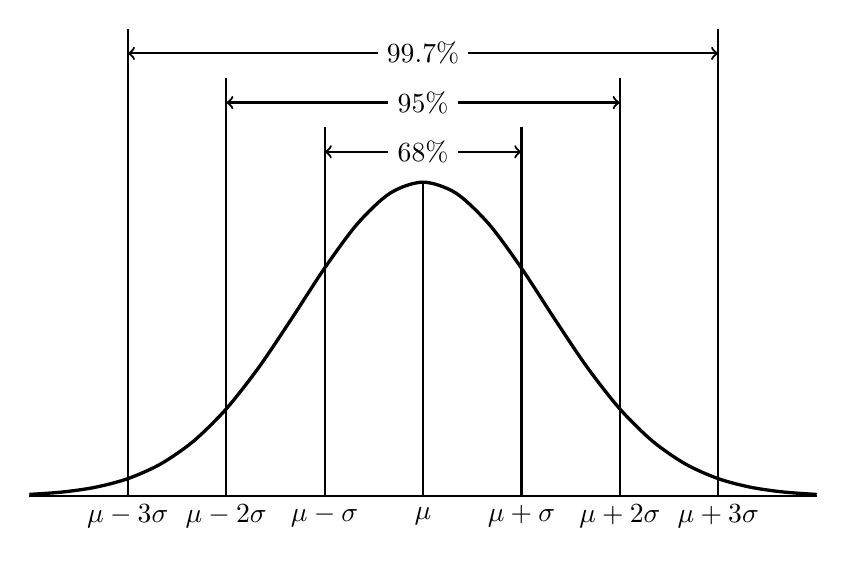
\begin{tikzpicture}[thick, domain=-4:4, scale=1.25]
	% axes
	\draw (-4, 0) -- (4, 0);
	\draw (+0, 0) -- (0, 3.18);
	\node at (-3, -0.2) {$\mu-3\sigma$};
	\node at (-2, -0.2) {$\mu-2\sigma$};
	\node at (-1, -0.2) {$\mu-\sigma$};
	\node at (+0, -0.2) {$\mu$};
	\node at (+1, -0.2) {$\mu+\sigma$};
	\node at (+2, -0.2) {$\mu+2\sigma$};
	\node at (+3, -0.2) {$\mu+3\sigma$};

	% gause function
	\def\gaussian#1#2{
		\draw[very thick, smooth] plot (\x, {10/(#2*sqrt(2*pi))*exp(-(\x-#1)^2/(2*#2^2))});
	}
	\gaussian{0}{1.25}

	% \percentage#std#y#percent
	\def\percentage#1#2#3{
		\draw (-#1, 0) -- (-#1, #2);
		\draw (+#1, 0) -- (+#1, #2);
		\draw[<->] (-#1, #2 - .25) -- (+#1, #2 - .25);
		\node[fill=white] at (0, #2 - .25) {#3\%};
	}
	\percentage{1}{3.75}{68}
	\percentage{2}{4.25}{95}
	\percentage{3}{4.75}{99.7}
\end{tikzpicture}